\chapter{Dr. Kellogg and the Trinity doctrine}

The key problem with the Kellogg controversy was the sentiments over the \emcap{personality of God}, which were departing from the foundation of our faith, that God established at the beginning of our work. We have been told that \egwinline{Many things of like character will in the future arise}[Ms137-1903.10; 1903][https://egwwritings.org/read?panels=p9939.17]. In the book, the Living Temple, we see the sentiments regarding the \emcap{personality of God} and where His presence is, which were stepping off of the \emcap{Fundamental Principles}. This step was never supposed to be made! But we raise the question, where was this step heading? We will see the evidence that this step was heading toward the Trinity doctrine. Sister White prophesied that Kellogg’s step would lead toward the Omega heresy. Can we see the connection between Kellogg’s controversy and the Trinity doctrine?

In the following section, we want to present you with the connection between Kellogg’s controversy and the doctrine of Trinity. It is important to emphasize that the Living Temple does not contain this doctrine as it is believed today. The main problem with Kellogg’s teaching was the \textit{stepping off} of the \emcap{Fundamental Principles}, which were the foundation of our faith. The information we will present to you reveals that Dr. Kellogg justified his actions in stepping off of the foundation through his belief in the doctrine of Trinity. This is not difficult to see when we recognize that the \emcap{Fundamental Principles} were a non-Trinitarian. Our main focus should not be in recognizing the Trinity doctrine in Kellogg's arguments, but rather in understanding the differences between Kellogg’s teachings and the teachings of the \emcap{Fundamental Principles} regarding \egwinline{the personality of God and where His presence is}[SpTB02 51.3; 1903][https://egwwritings.org/read?panels=p417.262]. In other words, what were the steps Kellogg made in stepping off of the foundation of our faith? This approach is advocated by the Spirit of Prophecy and it will help us to avoid speculations regarding Kellogg’s motives—it will help us to focus upon the truth. Ellen White tells us that there are many good things written in the Living Temple, but they are mingled with specious, deceptive theories regarding the \emcap{personality of God} and \emcap{of Christ}.

\begin{figure}[hp]
    \centering
    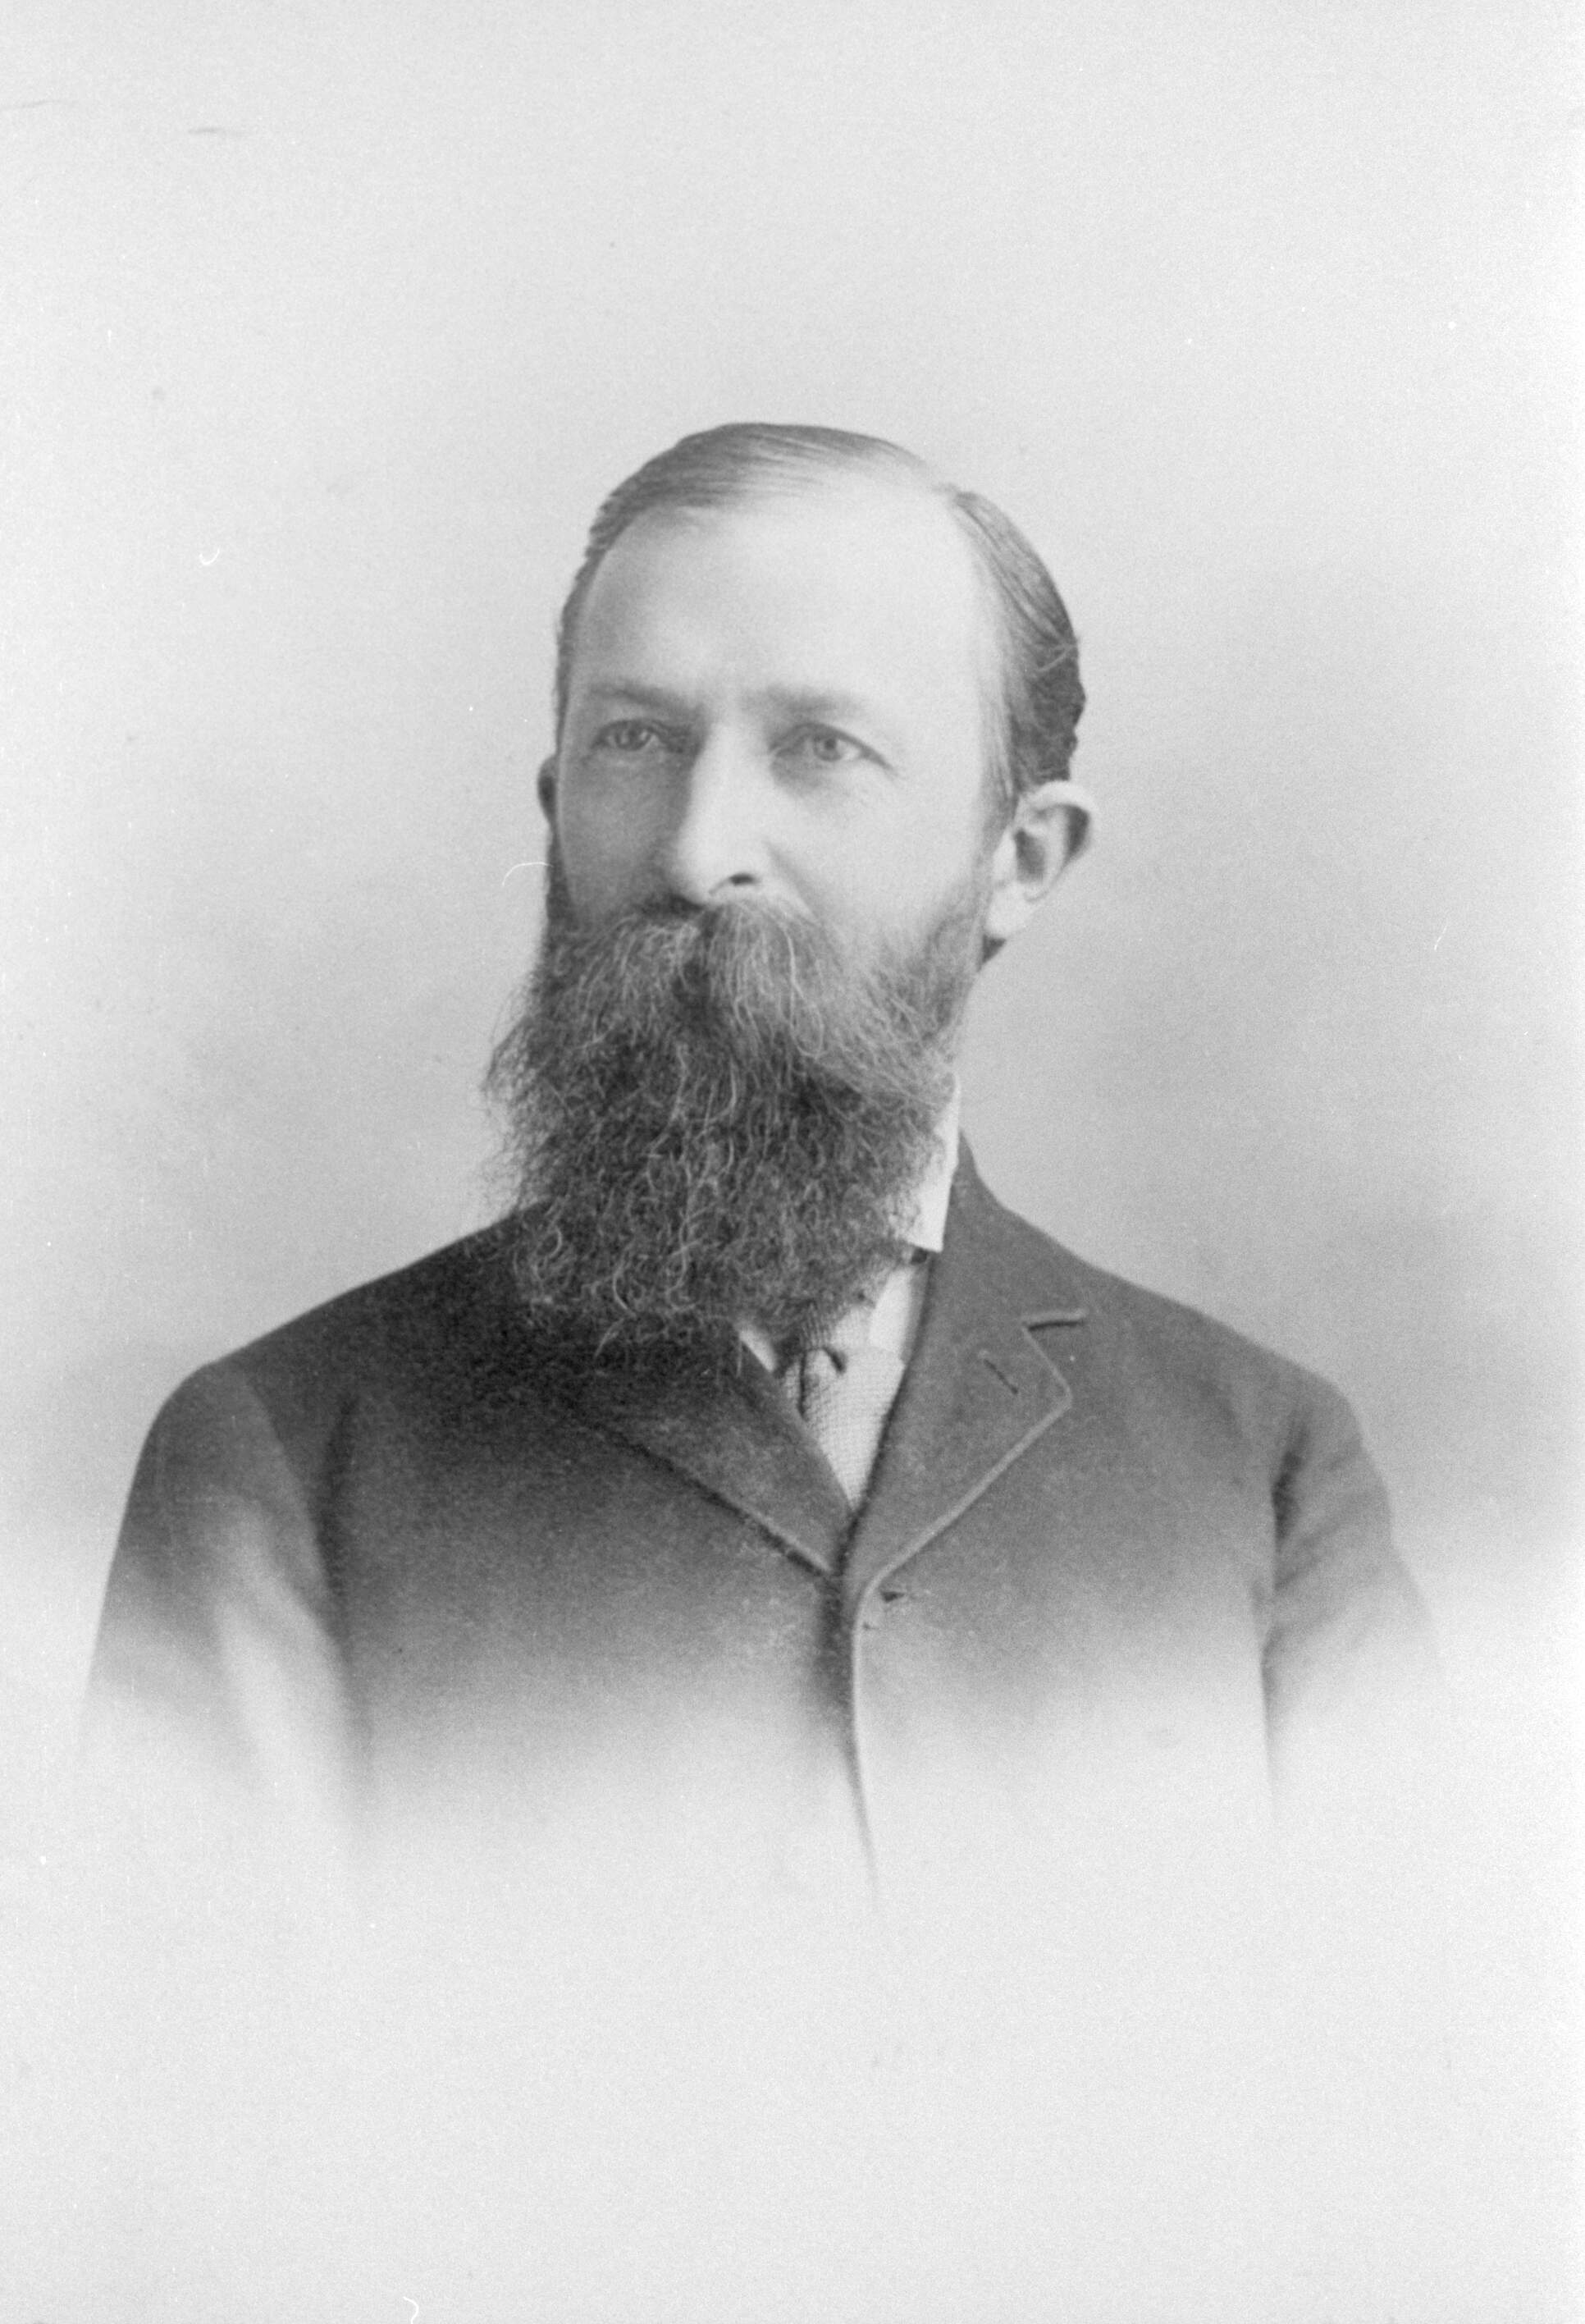
\includegraphics[width=1\linewidth]{images/john-h-kellogg.jpg}
    \caption*{John Harvey Kellogg (1852-1943)}
    \label{fig:john-h-kellogg}
\end{figure}

\egw{\textbf{The book Living Temple contains specious, \underline{deceptive sentiments regarding the personality of God and of Christ}}. The Lord opened before me the true meaning of these sentiments, showing me that unless they were steadfastly repudiated, they would deceive the very elect. \textbf{Precious truth and beautiful sentiments were woven in with false, misleading theories. Thus truth was used to substantiate the \underline{most dangerous errors}. The precious representations of God are so misconstrued as to appear to uphold falsehoods \underline{originated by the great apostate}. Sentiments that belong to the revealings of God are mingled with specious, deceptive theories of satanic agencies}.}[Lt146-1905.2; 1905][https://egwwritings.org/read?panels=p9430.8]

\egwnogap{In the controversy over these theories \textbf{it has been asserted that I believed and taught the same things} that I have been instructed to condemn in the book Living Temple. \textbf{This I deny}. In the name of Jesus Christ of Nazareth, \textbf{I say that this is not so}.}[Lt146-1905.3; 1905][https://egwwritings.org/read?panels=p9430.9]

This mixture of truth and error makes the matter difficult. In the eyes of pro-trinitarian scholars, the problem is solely attributed to pantheism, and the evidence of Kellogg's belief in the Trinity doctrine is interpreted as belief in a false Trinity\footnote{Whidden, Woodrow W, et al. \textit{The Trinity : Understanding God's Love, His Plan of Salvation, and Christian Relationships}. Hagerstown, Md, Review And Herald Pub. Association, 2002., p. 217}. Sister White's rebuke is attributed to the defense of the “correct” Trinity, which she supposedly believed. Unfortunately, such interpretation does not acknowledge Sister White's defense of the \emcap{Fundamental Principles} regarding the \emcap{personality of God} and of Christ, thus it is a misinterpretation of her work. In the following sections, we will examine historical data on Dr. Kellogg's connection with the doctrine of Trinity from the perspective of the Adventist truth on the \emcap{personality of God}, which constituted the foundation of our faith. With this perspective, we believe that the historical data will shine in a new light and spark honest and constructive dialogue in our church.

\section*{Correspondence of Dr. Kellogg and Brother Butler}

In the following section we briefly present you with the well-known correspondence between Dr. Kellogg and G. I. Butler over the book, the Living Temple. Here, we see Dr. Kellogg’s objections regarding the controversy. He wrote to Brother Butler:

\others{As far as I can fathom, the \textbf{difficulty }which is found \textbf{in ‘The Living Temple’,} \textbf{the whole thing may be simmered down to the question}: \textbf{\underline{Is the Holy Ghost a person}?} You say no. I had supposed the Bible said this for the reason that the personal pronoun ‘he’ is used in speaking of the Holy Ghost. \textbf{Sister White uses the pronoun ‘he’ and has said in so many words that the Holy Ghost is \underline{the third person of the Godhead}}. \textbf{How the Holy Ghost can be the third person and not be a person at all is difficult for me to see}.}[Letter: J. H. Kellogg to G. I. Butler. Oct 28. 1903][https://static1.squarespace.com/static/554c4998e4b04e89ea0c4073/t/5db9fbc96defed1e45b497a4/1572469707862/1903-10-28-Kellog-to-Butler.pdf]

\begin{figure}[hp]
    \centering
    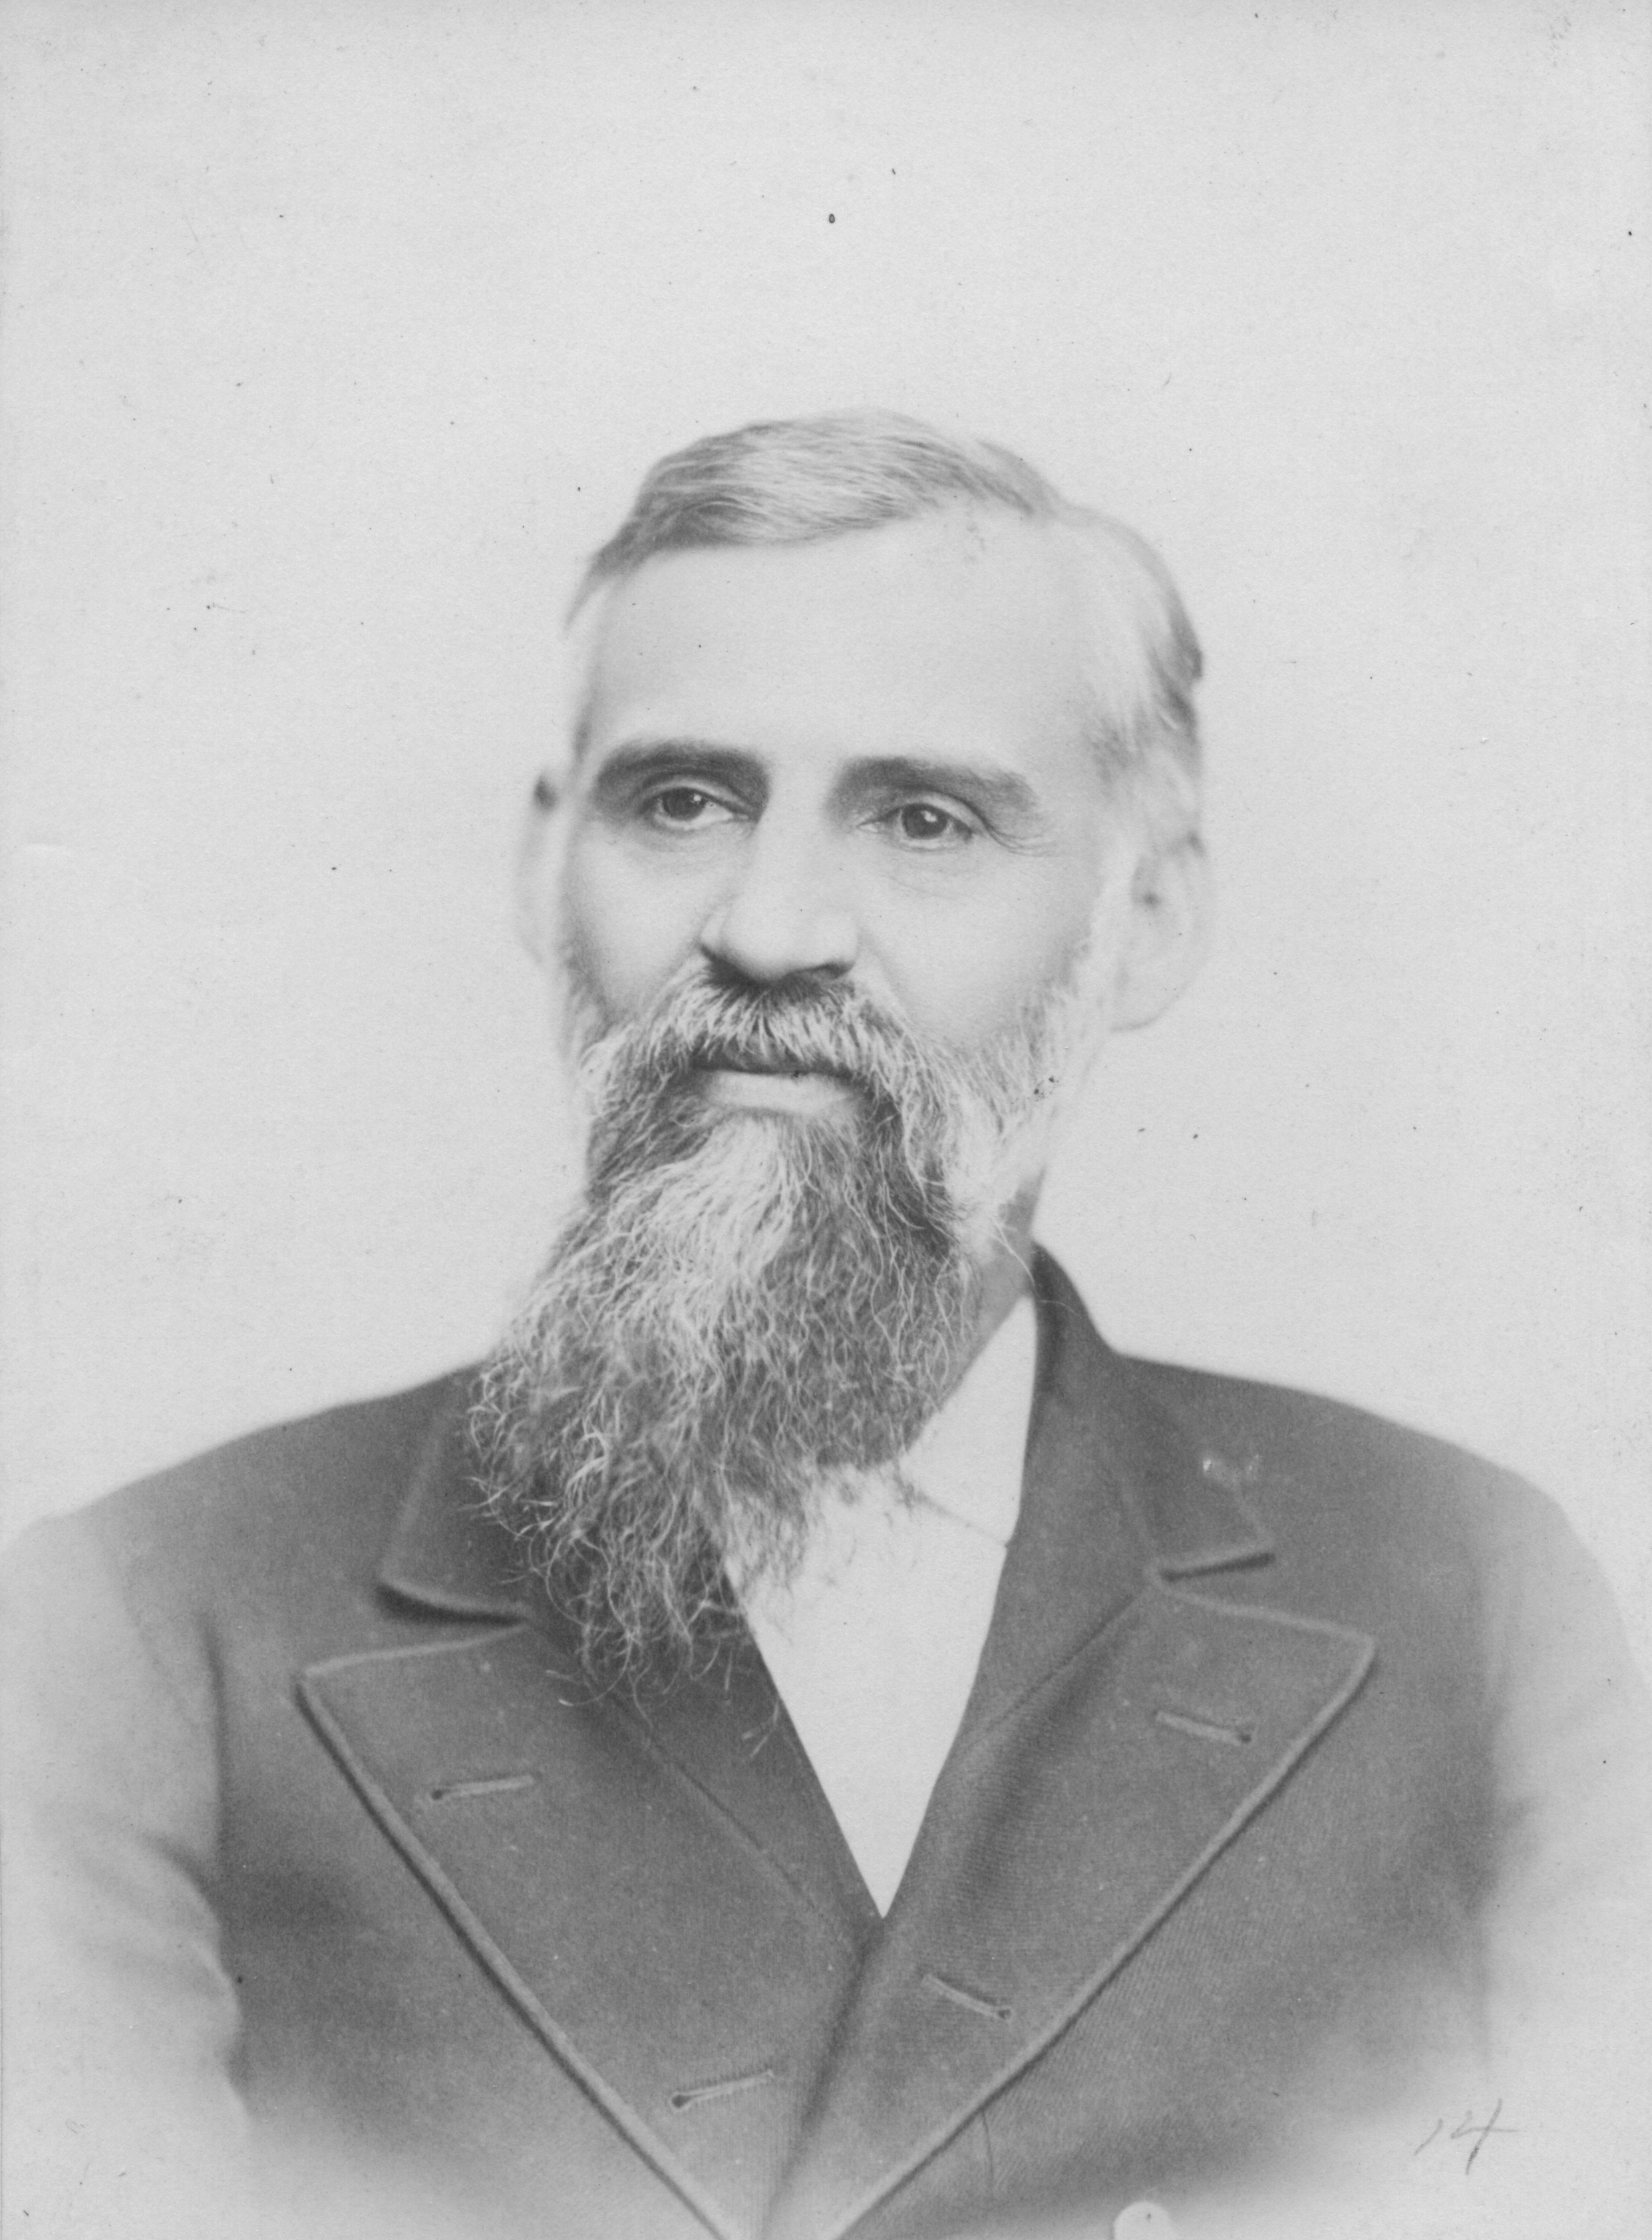
\includegraphics[width=1\linewidth]{images/george-ide-butler.jpg}
    \caption*{George Ide Butler (1834-1918)}
    \label{fig:g-i-butler}
\end{figure}

According to Dr. Kellogg’s perspective, the whole problem with the book ‘The Living Temple’ comes down to the question “\textit{Is the Holy Ghost a person?}”. Obviously, he does not advocate an impersonal God, as he is often accused of\footnote{Whidden, Woodrow W, et al. \textit{The Trinity : Understanding God's Love, His Plan of Salvation, and Christian Relationships}. Hagerstown, Md, Review And Herald Pub. Association, 2002., p. 217}. Moreover, he even believes that the Holy Ghost is a \textit{third person of the Godhead}. Also, he claims that Brother Butler does not believe that the Holy Ghost is a person. The problem obviously lies in the definition of the word \textit{‘person’}. On this point, Kellogg continues:

\others{I believe this Spirit of God to be a personality you don’t. But this is purely a question of definition. \textbf{I believe the Spirit of God is a personality}; you say, No, it is not a personality. Now the only reason why we differ is because we \textbf{differ in our ideas as to \underline{what a personality is}}. \textbf{Your idea of personality is perhaps that of \underline{semblance to a person} or a human being}.}[Letter: J. H. Kellogg to G. I. Butler. Oct 28. 1903][https://static1.squarespace.com/static/554c4998e4b04e89ea0c4073/t/5db9fbc96defed1e45b497a4/1572469707862/1903-10-28-Kellog-to-Butler.pdf]

Brother Butler replied:

\others{\textbf{So far as Sister White and you being in perfect agreement, I shall have to leave that entirely between you and Sister White. \underline{Sister White says there is not perfect agreement; you claim there is}. \underline{I know some of her remarks seem to give you strong ground for claiming that she does}. I am candid enough to say that, but I must give her the credit until she disowns it of saying there is a difference too, and I do not believe you can fully tell just what she means. \underline{God dwells in us by His Holy Spirit}, as a Comforter, as a Reprover, especially the former. When we come to Him we partake of Him in that sense, because the Spirit comes forth from Him; \underline{it comes forth from the Father and the Son}. It is not a person walking around on foot, or flying \underline{as a literal being}, \underline{in any such sense as Christ and the Father are} – at least, if it is, it is utterly beyond my comprehension of the meaning of language or words}.}[Letter: G. I. Butler to J. H. Kellogg. April 5. 1904]

The given correspondence is crucial for understanding the Kellogg controversy. Kellogg himself stated, \others{the whole thing may be simmered down to the question: \textbf{Is the Holy Ghost a person?}} Similarly Dr. Kellogg wrote to William White: \others{I have been studying very carefully to see what is \textbf{the real root of the difficulty with the Living Temple}, and as far as I can see \textbf{\underline{the whole question} resolves itself into this: \underline{Is the Holy Ghost, a person}?}}[Letter J. H. Kellogg to William White, October 28, 1903][https://drive.google.com/file/d/1\_S4S-Hc0K7Ka8gda9oRhPuAb9XzBTwmb/view] How does Kellogg's conclusion compare to the review and instruction of heavenly origin, which clearly told us that the reasoning in the Living Temple is \egwinline{naught but speculation in regard to \textbf{the personality of God and where His presence is}}[SpTB02 51.3; 1904][https://egwwritings.org/read?panels=p417.262]? In the writings of Ellen White and the pioneers, the term ‘\textit{personality of God}’ refers specifically to the personality of the Father. So, why does Kellogg claim that the real issue is the personality of the Holy Spirit, when God indicated that the issue concerns the personality of the Father?

Many assume that Dr. Kellogg is being manipulative, evading the core issue. However, under a particular premise, his arguments concerning the personality of the Holy Spirit logically support his controversial views on the \emcap{personality of God}. This premise becomes evident within the data itself when we closely follow his reasoning.

As we have seen earlier, the doctrine on the \emcap{personality of God} teaches that God, the Father, possesses a form—a tangible, material body. Dr. Kellogg concurred that this assertion holds true within the bounds of our finite conception of God\footnote{\href{https://archive.org/details/J.H.Kellogg.TheLivingTemple1903/page/n33/}{Dr. John H. Kellogg, The Living Temple, p.31.}}. However, he argued that, in reality, God transcends our conceptions regarding His form, as He is beyond the constraints of space\footnote{\href{https://archive.org/details/J.H.Kellogg.TheLivingTemple1903/page/n33/}{Dr. John H. Kellogg, The Living Temple, p.33.}}. In this sense, Kellogg effectively does away with the reality of God’s physical, material body. The premise that would validate Dr. Kellogg’s viewpoint is the \textit{exclusive equivalence} in understanding the \emcap{personality of God} and that of the Holy Spirit. Is the Holy Spirit constrained by space? No, He is not. Does the Holy Spirit have a physical body? No! According to Jesus, \bible{for a spirit hath not flesh and bones}[Luke 24:39]. Is the Holy Ghost a person? The answer hinges on our interpretation of what it means to be a person. What is that quality or state of the Holy Spirit being a person?\footnote{Direct application of the definition on the word ‘\textit{personality}’ from the \href{https://www.merriam-webster.com/dictionary/personality}{Merriam Webster Dictionary}} When comparing Dr. Kellogg's belief in the personality of the Holy Spirit with Brother Butler's views, it becomes evident that the quality of the Holy Spirit being a person does not align with \others{that of \textbf{semblance to a person} or a human being}. Butler explicitly stated his criteria for this determination\footnote{In his letter to Dr. Kellogg, Brother Butler further asserted that there is no distinction between the person and the bodily presence. See \href{https://c7da.us/egwdl/Butler\%20to\%20Kellogg\%20Aug121904.pdf}{Letter from Butler to Kellogg, August 12, 1904, p.6}}: \others{\textbf{It is not a person walking around on foot, or flying \underline{as a literal being}, \underline{in any such sense as Christ and the Father are} – at least, if it is, it is utterly beyond my comprehension of the meaning of language or words}}.

Have you noticed that Brother Butler addressed Kellogg’s unspoken premise? Butler drew a distinction between the Father and Christ, in relation to the Holy Spirit. Brother Butler is correct. There exists a contrast between the personality of the Holy Spirit and that of God and Christ. Christ and the Father possess a physical form of a person, whereas the Holy Spirit does not. To do away with the physical form of a person of the Father is to \textit{exclusively equate} the understanding of the personality of the Father with that of the Holy Spirit. Kellogg’s approach is compelling, because it was backed by valid arguments regarding the personality of the Holy Spirit.

Let us briefly examine the personality of the Holy Spirit. What is the quality or state of the Holy Spirit being a person?

\egw{\textbf{The Holy Spirit has a personality}, \textbf{\underline{else} }He could not \textbf{bear witness} to our spirits and with our spirits that we are the children of God. \textbf{He must also be a \underline{divine person}}, \textbf{\underline{else}} He could not \textbf{search out the secrets} which lie hidden \textbf{in the mind of God}.}[21LtMs, Ms 20, 1906, par. 32; 1906][https://egwwritings.org/read?panels=p14071.10296041&index=0]

\egw{\textbf{The Holy Spirit is a person}; \textbf{\underline{for}} He \textbf{beareth witness} with our spirits that we are the children of God.}[21LtMs, Ms 20, 1906, par. 31; 1906][https://egwwritings.org/read?panels=p14071.10296040&index=0]

The qualities or states that define the Holy Spirit as a person are explicitly mentioned in the provided quotations. These include the ability to bear witness and search out the mind. Further support can be found in Scripture, which attributes actions to the Holy Spirit such as speaking (\textit{Acts 13:2}), teaching (\textit{John 14:26; 1 Corinthians 2:13}), making decisions (\textit{Acts 15:28}), and experiencing emotions (\textit{Ephesians 4:30}), among others. These \textit{qualities }collectively affirm the personality of the Holy Spirit. Can these same qualities be also applied to the Father and the Son? Most certainly. However, unlike the Father and the Son, the Holy Spirit is distinguished by the absence of a material, tangible form. When Ellen White questioned Christ about the \emcap{personality of God}, her inquiry specifically targeted the personal form as the defining quality of the Father's personality.

\egw{I have often \textbf{seen }the lovely Jesus, that \textbf{He is a person}. \textbf{I asked Him if His Father \underline{was a person} and \underline{had a form} like Himself}. Said Jesus, ‘\textbf{I am in the express image of My Father's person}.’}[EW 77.1; 1882][https://egwwritings.org/read?panels=p28.490&index=0]

This brings us to a profound distinction in how the personality of the Holy Spirit is understood, as opposed to that of the Father and the Son. Ellen White describes the Holy Spirit as a spiritual manifestation of Christ, drawing a clear line between the outward, visible manifestation of Christ and His spiritual manifestation. This contrast underscores the unique nature of the Holy Spirit's presence and action in the world, distinct from the physical presence of Christ and the Father. Pay attention to the contrast between the outward, visible manifestation of Christ, and His spiritual manifestation:

\egw{That \textbf{Christ }should \textbf{manifest Himself} to them, and yet \textbf{be invisible to the world}, was a mystery to the disciples. They could not understand \textbf{the words of Christ in their \underline{spiritual sense}}. \textbf{They were thinking of \underline{the outward, visible manifestation}}. They could not take in the fact that they could have \textbf{the presence of Christ with them}, and \textbf{yet He be unseen by the world}. \textbf{They did not understand the meaning of \underline{a spiritual manifestation}}.}[ST November 18, 1897, par. 6; 1897][https://egwwritings.org/read?panels=p820.14727&index=0]

The Holy Spirit is not a person in the physical sense but is manifested in a spiritual sense. If the exclusive understanding of the personality of the Holy Spirit is applied to the Father, then consequently His physical form of a person is done away. His personality is spiritualized. This is why Ellen White critically labeled Kellogg's perspective as spiritualism. Do you know which doctrine, in particular, has a core tenet, that the Father and the Holy Spirit are co-equal in their personalities? It is \textit{the doctrine of the trinity}. Could it be possible that Dr. Kellogg was actually raising the theological side of questions of the trinity?

\section*{Kellogg’s confession about the Living Temple}

In his interview with G. W. Amadon and A. C. Bourdeau, one month after being disfellowshipped, he confessed that he unintentionally brought the theological side of the question of the Trinity into his book “The Living Temple”.

\others{\textbf{Now, I thought I had cut out entirely the theological side of questions of \underline{the trinity and all that sort of things}}. \textbf{I didn't mean to \underline{put it in} at all}, and I took pains to state in the preface that I did not. I never dreamed of such a thing as \textbf{any theological question being} \textbf{\underline{brought into it}}. I only wanted to show that \textbf{the heart does not beat of its own motion but that it is the power of God that keeps it going}.}[Kellogg vs. The Brethren: His Last Interview as an Adventist, p. 58.][https://forgotten-pillar.s3.us-east-2.amazonaws.com/1990\_kellogg\_vs\_brethren\_lastInterview\_oct7\_1907\_spectrum\_v20\_n3-4.pdf]

If we were to look in his book for trinitarian expressions, we would not find any. Would that be a proof that Kellogg is disingenuous in his confession? The only thing we find is the teaching that is stepping off of the foundation of our faith—the \emcap{fundamental principles}—regarding the \emcap{personality of God} and where His presence is. The trinitarian expressions are not there but his sentiments regarding the \emcap{personality of God} are in line with the trinitarian sentiments on God’s person. These sentiments are deceptive and Kellogg was rebuked for them. When he wanted to explicitly state the belief in the Trinity doctrine, in hopes of fixing the book, he was again rebuked by the words, \egwinline{\textbf{Patchwork theories} cannot be accepted by those who are loyal to the faith} and to the \emcap{Fundamental Principles}\footnote{\href{https://egwwritings.org/?ref=en_Lt253-1903.28&para=9980.36}{EGW, Lt253-1903.28; 1903}}. The crucial problem of the Trinity doctrine, in regard to the \emcap{personality of God}, is the underlying assumption that all Three, the Father, the Son, and the Holy Spirit, possess the same type of personality in such a way that They make one monotheistic God. In this light, we may understand Kellogg's assertions over the personality of the Holy Spirit, that the Holy Spirit is the third person of the Godhead. Dr. Kellogg quoted Ellen White when asserting his claims; although he used the same words, he had a wrong sentiment. In light of Dr. Kellogg’s confession, for including \others{\textbf{the theological side of questions of \underline{the trinity}}}, and His assertion that \others{\textbf{the whole thing may be simmered down to the question}: \textbf{\underline{Is the Holy Ghost a person}}?}, we may see the unspoken premise that the Father and the Son are in the same way persons as is the Holy Spirit. This is why Brother Butler wrote to him regarding the personality of the Holy Spirit: \others{\textbf{It is not a person walking around on foot, or flying \underline{as a literal being}, \underline{in any such sense as Christ and the Father are} – at least, if it is, it is utterly beyond my comprehension of the meaning of language or words.}}[Letter from G. I. Butler to J. H. Kellogg, April 5 1904.]


\section*{The presence of God manifested in nature}

From the works of our pioneers, we have seen that the personality of the Holy Ghost is most clearly expressed in terms of God's presence. Sister White told us that the Living Temple \egwinline{introduces that which is naught but speculation in \textbf{regard to the personality of God and where His presence is}.}[SpTB02 51.3; 1904][https://egwwritings.org/read?panels=p417.262] The \emcap{personality of God} and where His presence is are two mutually inclusive doctrines; one affirms the other. Deny one, and you deny the other. This notion is clearly seen in the book, the Living Temple. In the previous sections, we read Kellogg's arguments for the \emcap{personality of God} taken from his book. He argued that it is unprofitable to talk about God's shape or any tangible form. He raised skepticism in the reality of God as a definite, material, and tangible Being. If God is spirit, possessing no form nor body, then He is not restricted in His presence to one locality; this was the sentiment Kellogg advocated in the Living Temple.

\others{Says one, ‘\textbf{God may be \underline{present by his Spirit}, or by his power, but \underline{certainly God himself} cannot be present everywhere at once}.’ We answer: How can power be separated from the source of power? \textbf{Where God's Spirit is at work}, where God's power is manifested, \textbf{God \underline{himself} is actually and truly present}…}[John H. Kellogg, The Living Temple, p.28.][https://archive.org/details/J.H.Kellogg.TheLivingTemple1903/page/n29/]

When Dr. Kellogg wrote \others{Says one, ‘God may be present by His Spirit…’}, he referred to the sentiments of our pioneers who were loyal to the \emcap{Fundamental Principles}. This is the most obvious point where Dr. Kellogg stepped off from the \emcap{Fundamental Principles}. Is this step in harmony with the doctrine of the Trinity? Examining our current stance in the Fundamental Beliefs \#2, we see that one God, as a unity of three persons, is not everywhere present through the agency of the Holy Spirit, but rather is everywhere present by Himself.

\others{There is \textbf{one God}: Father, Son, and Holy Spirit, \textbf{a unity of three} coeternal \textbf{Persons}. God is immortal, all-powerful… and \textbf{ever present}.}[Fundamental Beliefs of Seventh-day Adventist, \#2 Trinity; 2020 Edition][https://www.adventist.org/wp-content/uploads/2020/06/ADV-28Beliefs2020.pdf]

\section*{Dr. Kellogg's perception of God}

In examining the surrounding controversy over the Living Temple, we truly see that Dr. Kellogg raised \others{the theological side of questions of the trinity.}[Kellogg vs. The Brethren: His Last Interview as an Adventist, p. 58.][https://forgotten-pillar.s3.us-east-2.amazonaws.com/1990\_kellogg\_vs\_brethren\_lastInterview\_oct7\_1907\_spectrum\_v20\_n3-4.pdf] Another question we raise in examining Kellogg's sentiments with the \emcap{Fundamental Principles} is whom does he address in terms of “\textit{one God}”? There is no data to directly answer that question, but there is plenty of data which suggests that Dr. Kellogg's understanding of “\textit{one God}” was a Trinitarian understanding. His letter to W. W. Prescott is one piece of evidence supporting that notion:

\others{The difference is this: \textbf{When we say God} is in the tree, the word ‘\textbf{God}’ \textbf{is understood in its most comprehensive sense}, and people understand the meaning to be \textbf{that the Godhead} is in the tree, \textbf{God the Father, God the Son, and God the Holy Spirit}, whereas the proper understanding in order \textbf{that wholesome conceptions} should be preserved in our minds, is that God the Father sits upon his throne in heaven where God the Son is also; \textbf{while God's life, or spirit or presence is the all-pervading power which is carrying out the will of God in all the universe}.}[Letter: Dr. Kellogg to Prof. W. W. Prescott, Oct. 25, 1903][https://forgotten-pillar.s3.us-east-2.amazonaws.com/1903-10-25-JHKellogg-to-W.W.Prescott.pdf]

In the next chapter, we will make our case: if the given \others{wholesome conception} of God advocated by Dr. Kellogg was true, then his clarification of the Holy Spirit being \others{God's life, or spirit or presence is the all-pervading power which is carrying out the will of God in all the universe} would truly solve the entire difficulty of the Living Temple. But that was not the case. Dr. Kellogg's true problem was his perception of God, and his trinitarian stance was not solving the real issue—the \emcap{personality of God}.

There is another revealing letter showing us the consequences of raising \others{the theological side of questions of the trinity.} Writing to his friend Dr. Hayward, Dr. Kellogg reflected:

\others{\textbf{These theologians} have sought to darken the minds of the people and to make \textbf{this sweet and beautiful truth \underline{appear loathsome} to them, by drawing into it \underline{the old controversy about the Trinity}}.}

\othersnogap{I never raised the question as to \textbf{which part of God is present in a man}, whether it was \textbf{God, the Father};\textbf{ God, the Son}; or \textbf{God, the Holy Spirit}. The only point was that it is God and not man.}[Letter: Dr. J. H. Kellogg to Dr. Hayward, Aug., 15. 1905][https://forgotten-pillar.s3.us-east-2.amazonaws.com/1903-08-15-kellogg-to-hayward.pdf]

Here we see the tensions between Dr. Kellogg and certain Seventh-day Adventist theologians of that time, where Dr. Kellogg's \others{sweet and beautiful truth} of God's divine immanence got entangled with \others{the old controversy about the Trinity}. This tells us that in the days of Dr. Kellogg, the doctrine of Trinity was controversial, and certainly it was not regarded as something positive, but rather as something which made Kellogg's teachings \others{loathsome}. But who were these theologians Dr. Kellogg referred to? He did not name anyone in his letter to Dr. Hayward, but we can get the idea of whom \others{these theologians} were based on his letter sent 10 days earlier to I. G. Butler\footnote{\href{https://forgotten-pillar.s3.us-east-2.amazonaws.com/1905-08-05-kellogg-butler.pdf}{Letter: J. H. Kellogg to I. G. Butler, Aug., 5. 1905}}, venting his frustration with the General Conference's bidding with him. These were A. G. Daniells, W. C. White, and W. W. Prescott. We can also include G. I. Butler himself to that group, since he also was a theologian participating in this \others{old controversy about the Trinity}. All of these people held leading positions within the Seventh-day Adventist church, and all of them were non-Trinitarians. The argument is being made that the issue with Dr. Kellogg's teaching lies somewhere other than his trinitarian sentiments, because supposedly the church was trinitarian at that time, and supposedly Ellen White was trinitarian herself. \footnote{This is currently the popular narrative promoted by laity.} If this was the case, and in this mix of truth and error, should we not have at least some defense of the trinity doctrine, dissecting it from error? We have not found any such data. Instead, all data we have is in defense of the \emcap{Fundamental Principles}, and the doctrine on the presence and the \emcap{personality of God}, which both are opposed to the doctrine of the Trinity. Ellen White said of the truth: the Trinity doctrine \egwinline{cannot be accepted by those who are \textbf{loyal to the faith and to the principles} that have withstood all the opposition of satanic influences.}[Lt253-1903.28; 1903][https://egwwritings.org/read?panels=p14068.9980036]

In this short reflection on differences between Dr. Kellogg's sentiments and the \emcap{Fundamental Principles} from which he stepped off, we can recognize the following characteristics which are akin to the Trinity doctrine:

\begin{itemize}
    \item The word ‘God’ represents the wholesome conception of God as God the Father, God the Son, and God the Holy Spirit.
    \item God is everywhere present by Himself.
    \item The quality or state of the Father being a person is equalized to that of the Holy Spirit.\footnote{\href{https://www.adventist.org/wp-content/uploads/2020/06/ADV-28Beliefs2020.pdf}{Fundamental Beliefs \#5}: \others{He \normaltext{[the Holy Spirit]} \textbf{is as much a person} \underline{as} are \textbf{the Father} and the Son}; \href{https://www.adventist.org/wp-content/uploads/2020/06/ADV-28Beliefs2020.pdf}{Fundamental Beliefs \#3}: \others{\textbf{The qualities} and powers \textbf{exhibited in} the Son and \textbf{the Holy Spirit are \underline{also} those of the Father}}}
\end{itemize}

These three characteristics of Dr. Kellogg's sentiments depart from the foundation of our faith—the \emcap{Fundamental Principles}—but are in harmony with the teachings of the Trinity. In saying this, we are not claiming that Dr. Kellogg is responsible for the acceptance of the Trinity doctrine into our ranks, but rather that the Trinity doctrine was Kellogg's justification for stepping off from the foundation of our faith, established at the beginning of our work. The true problem was \textit{stepping off} from the \emcap{fundamental principles}, and both Dr. Kellogg and we as a church have made those steps. The difference is that Dr. Kellogg landed in pantheism, while we landed on the \#2 point of the Fundamental Beliefs.

In the following chapter, we will examine Dr. Kellogg's teaching that God sustains all life, and how this truth, in combination with a false perception of God and His personality, led him to become a pantheist.

% Dr. Kellogg and the Trinity doctrine

\begin{titledpoem}
    
    \stanza{
        In Kellogg's quest, a question posed, \\
        "Is the Holy Ghost, indeed, a person enclosed?" \\
        A controversy stirred, the essence debated, \\
        The Trinity's mystery, intricately related.
    }

    \stanza{
        Kellogg questioned beyond the tangible, the seen, \\
        Where the Holy Spirit's form has never been. \\
        A spiritual essence, not bound by space, \\
        Challenging the Father's physical embrace.
    }

    \stanza{
        The Holy Ghost, a person, yet not in form, \\
        In actions, emotions, a divine norm. \\
        Witnessing, teaching, decisions so clear, \\
        A presence felt, though not seen near.
    }

    \stanza{
        Butler contrasted, in physical sense, \\
        The Father and Christ, their presence immense. \\
        Yet, the Spirit's persona, distinct in its role, \\
        A spiritual manifestation, completing the whole.
    }

    \stanza{
        Ellen asked of Jesus, if His Father's form was like His own, \\
        "In my Father's image," He replied, in a tone so gently sown. \\
        Yet, the Spirit, in essence, a guiding light, \\
        Not seen, but felt, in the believers' sight.
    }

    \stanza{
        A doctrine emerges, the Trinity's core, \\
        Equal in personalities, yet so much more. \\
        Kellogg's perspective, once seen as stray, \\
        Raises the question, in a theological way.
    }

    \stanza{
        Yet, Scripture guides, through mystery's veil, \\
        Revealing God's form, where human views fail. \\
        The Father, embodied, a truth we embrace, \\
        While the Spirit's presence, a formless grace.
    }

    \stanza{
        In divine revelation, the answers found, \\
        God's personality, in Scripture, profound. \\
        The Father, in form; the Spirit, without, \\
        In this, the Bible resolves all doubt.
    }
\end{titledpoem}